\documentclass[tikz]{standalone}

\usetikzlibrary{shapes,arrows,shadows,calc, angles}
\usetikzlibrary{arrows,shapes}
\usetikzlibrary{positioning}
\usetikzlibrary{patterns.meta}
\usetikzlibrary{decorations, decorations.pathreplacing}

\definecolor{fg}{rgb}{0,0,0}
\definecolor{bg}{rgb}{1,1,1}

\tikzstyle{box}=[draw, rounded corners , text width=40mm,
anchor=center,text centered,text=fg, font=\bfseries] % text width=33mm,

\tikzstyle{myarrow}=[->, >=stealth, very thick, rounded corners=2mm]
\tikzstyle{mythinarrow}=[myarrow, line width=0.25mm]

\tikzstyle{conv}=[box, fill=red!60]
\tikzstyle{norm}=[box, fill=yellow!60]
\tikzstyle{upsample}=[box, fill=green!60]


\begin{document}

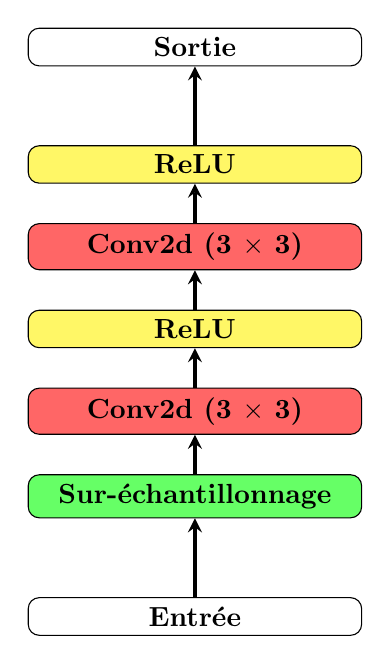
\begin{tikzpicture}

    \node[box] (X) {Entrée};
    
    \node[upsample, above=of X] (up1) {Sur-échantillonnage} ;
    \draw[myarrow] (X) -- (up1) ;
    
    \node[conv, above=of up1, yshift=-5mm] (conv1) {Conv2d (3~$\times$~3)} ;
    \draw[myarrow] (up1) -- (conv1) ;
    
    \node[norm, above=of conv1, yshift=-5mm] (norm1) {ReLU} ;
    \draw[myarrow] (conv1) -- (norm1) ;

    \node[conv, above=of norm1, yshift=-5mm] (conv2) {Conv2d (3~$\times$~3)} ;
    \draw[myarrow] (norm1) -- (conv2) ;
    
    \node[norm, above=of conv2, yshift=-5mm] (norm2) {ReLU} ;
    \draw[myarrow] (conv2) -- (norm2) ;
    
    \node[box, above=of norm2] (Y) {Sortie};
    \draw[myarrow] (norm2) -- (Y) ;
    

    % \node[conv, below=of norm1, yshift=5mm] (conv2) {Conv2d (3~$\times$~3), stride} ;
    % \draw[myarrow] (norm1) -- (conv2) ;

    % \node[norm, below=of conv2, yshift=5mm] (norm2) {Batch Norm et ReLU} ;
    % \draw[myarrow] (conv2) -- (norm2) ;

    % \node[conv, below=of norm2, yshift=5mm] (conv3) {Conv2d (1~$\times$~1)} ;
    % \draw[myarrow] (norm2) -- (conv3) ;
    
    % \node[draw, circle, minimum height= 5mm, below=of conv3, yshift=5mm] (add) {+} ;
    % \draw[myarrow] (conv3) -- (add) ;
    % \draw[myarrow] (X) -- ++ (0, -7mm) -| ++ (-25mm, -15mm) |- (add) ;
    % \node[box, below=of add, yshift=5mm] (Y) {sortie} ;
    % \draw[myarrow] (add) -- (Y) ;
\end{tikzpicture}

\end{document}